\newpage
\section{Teilversuch 2: Drehmoment des Feldes auf eine stromdurchflossene Spule}
	Fehler bei der Winkelmessung $\Delta \alpha = \SI{2}{\degree}$ \\
	Fehler bei der Winkelmessung $\Delta \beta = \SI{1.0}{\degree}$
 	\begin{equation*}
 		\begin{tabu}{l *{10}{l}}
 			\toprule
 			\alpha / \si{\degree} & 0 & 10 & 20 & 30 & 40 & 50 & 60 & 70 & 80 & 90 \\
 			\midrule
			\beta/ \si{\degree} & 295,0 & 315,0 & 337,0 & 358,5 & 377,0 & 395,0 & 413,0 & 425,5 & 437,5 & 449,0 \\
			(\beta - \beta_0)/ \si{\degree} & 0,0 & 20,0 & 42,0 & 63,5 & 82,0 & 100,0 & 118,0 & 130,5 & 142,5 & 154,0 \\
			\varphi / \si{\degree} & 0,0 & -10,0 & -22,0 & -33,5 & -42,0 & -50,0 & -58,0 & -60,5 & -62,5 & -64,0 \\
			\bottomrule
 		\end{tabu}
 	\end{equation*}
	wobei $\varphi = \alpha - (\beta - \beta_0)$.

	$\varphi$ wurde dann gegen $\sin (\alpha/\si{\degree})$ im \gnuplot{} geplottet und eine Kurveanpassung zur $\varphi = m\sin \alpha + c$ durchgeführt. 
	\begin{figure}[H]
		\centering
		% GNUPLOT: LaTeX picture with Postscript
\begingroup
  \makeatletter
  \providecommand\color[2][]{%
    \GenericError{(gnuplot) \space\space\space\@spaces}{%
      Package color not loaded in conjunction with
      terminal option `colourtext'%
    }{See the gnuplot documentation for explanation.%
    }{Either use 'blacktext' in gnuplot or load the package
      color.sty in LaTeX.}%
    \renewcommand\color[2][]{}%
  }%
  \providecommand\includegraphics[2][]{%
    \GenericError{(gnuplot) \space\space\space\@spaces}{%
      Package graphicx or graphics not loaded%
    }{See the gnuplot documentation for explanation.%
    }{The gnuplot epslatex terminal needs graphicx.sty or graphics.sty.}%
    \renewcommand\includegraphics[2][]{}%
  }%
  \providecommand\rotatebox[2]{#2}%
  \@ifundefined{ifGPcolor}{%
    \newif\ifGPcolor
    \GPcolortrue
  }{}%
  \@ifundefined{ifGPblacktext}{%
    \newif\ifGPblacktext
    \GPblacktexttrue
  }{}%
  % define a \g@addto@macro without @ in the name:
  \let\gplgaddtomacro\g@addto@macro
  % define empty templates for all commands taking text:
  \gdef\gplbacktext{}%
  \gdef\gplfronttext{}%
  \makeatother
  \ifGPblacktext
    % no textcolor at all
    \def\colorrgb#1{}%
    \def\colorgray#1{}%
  \else
    % gray or color?
    \ifGPcolor
      \def\colorrgb#1{\color[rgb]{#1}}%
      \def\colorgray#1{\color[gray]{#1}}%
      \expandafter\def\csname LTw\endcsname{\color{white}}%
      \expandafter\def\csname LTb\endcsname{\color{black}}%
      \expandafter\def\csname LTa\endcsname{\color{black}}%
      \expandafter\def\csname LT0\endcsname{\color[rgb]{1,0,0}}%
      \expandafter\def\csname LT1\endcsname{\color[rgb]{0,1,0}}%
      \expandafter\def\csname LT2\endcsname{\color[rgb]{0,0,1}}%
      \expandafter\def\csname LT3\endcsname{\color[rgb]{1,0,1}}%
      \expandafter\def\csname LT4\endcsname{\color[rgb]{0,1,1}}%
      \expandafter\def\csname LT5\endcsname{\color[rgb]{1,1,0}}%
      \expandafter\def\csname LT6\endcsname{\color[rgb]{0,0,0}}%
      \expandafter\def\csname LT7\endcsname{\color[rgb]{1,0.3,0}}%
      \expandafter\def\csname LT8\endcsname{\color[rgb]{0.5,0.5,0.5}}%
    \else
      % gray
      \def\colorrgb#1{\color{black}}%
      \def\colorgray#1{\color[gray]{#1}}%
      \expandafter\def\csname LTw\endcsname{\color{white}}%
      \expandafter\def\csname LTb\endcsname{\color{black}}%
      \expandafter\def\csname LTa\endcsname{\color{black}}%
      \expandafter\def\csname LT0\endcsname{\color{black}}%
      \expandafter\def\csname LT1\endcsname{\color{black}}%
      \expandafter\def\csname LT2\endcsname{\color{black}}%
      \expandafter\def\csname LT3\endcsname{\color{black}}%
      \expandafter\def\csname LT4\endcsname{\color{black}}%
      \expandafter\def\csname LT5\endcsname{\color{black}}%
      \expandafter\def\csname LT6\endcsname{\color{black}}%
      \expandafter\def\csname LT7\endcsname{\color{black}}%
      \expandafter\def\csname LT8\endcsname{\color{black}}%
    \fi
  \fi
    \setlength{\unitlength}{0.0500bp}%
    \ifx\gptboxheight\undefined%
      \newlength{\gptboxheight}%
      \newlength{\gptboxwidth}%
      \newsavebox{\gptboxtext}%
    \fi%
    \setlength{\fboxrule}{0.5pt}%
    \setlength{\fboxsep}{1pt}%
\begin{picture}(8640.00,5760.00)%
    \gplgaddtomacro\gplbacktext{%
      \csname LTb\endcsname%%
      \put(682,704){\makebox(0,0)[r]{\strut{}$25$}}%
      \put(682,1192){\makebox(0,0)[r]{\strut{}$26$}}%
      \put(682,1681){\makebox(0,0)[r]{\strut{}$27$}}%
      \put(682,2169){\makebox(0,0)[r]{\strut{}$28$}}%
      \put(682,2657){\makebox(0,0)[r]{\strut{}$29$}}%
      \put(682,3146){\makebox(0,0)[r]{\strut{}$30$}}%
      \put(682,3634){\makebox(0,0)[r]{\strut{}$31$}}%
      \put(682,4122){\makebox(0,0)[r]{\strut{}$32$}}%
      \put(682,4611){\makebox(0,0)[r]{\strut{}$33$}}%
      \put(682,5099){\makebox(0,0)[r]{\strut{}$34$}}%
      \put(814,484){\makebox(0,0){\strut{}$-100$}}%
      \put(1489,484){\makebox(0,0){\strut{}$0$}}%
      \put(2165,484){\makebox(0,0){\strut{}$100$}}%
      \put(2840,484){\makebox(0,0){\strut{}$200$}}%
      \put(3515,484){\makebox(0,0){\strut{}$300$}}%
      \put(4191,484){\makebox(0,0){\strut{}$400$}}%
      \put(4866,484){\makebox(0,0){\strut{}$500$}}%
      \put(5542,484){\makebox(0,0){\strut{}$600$}}%
      \put(6217,484){\makebox(0,0){\strut{}$700$}}%
      \put(6892,484){\makebox(0,0){\strut{}$800$}}%
      \put(7568,484){\makebox(0,0){\strut{}$900$}}%
      \put(8243,484){\makebox(0,0){\strut{}$1000$}}%
    }%
    \gplgaddtomacro\gplfronttext{%
      \csname LTb\endcsname%%
      \put(209,2901){\rotatebox{-270}{\makebox(0,0){\strut{}Temperatur $\theta$ ($\si{\celsius}$)}}}%
      \put(4528,154){\makebox(0,0){\strut{}Zeit $t$ ($\si{\second}$)}}%
      \csname LTb\endcsname%%
      \put(946,4893){\makebox(0,0)[l]{\strut{}$0,00832t + 25,66397$}}%
      \csname LTb\endcsname%%
      \put(946,4607){\makebox(0,0)[l]{\strut{}Messpunkte}}%
      \csname LTb\endcsname%%
      \put(4528,5429){\makebox(0,0){\strut{}Erwärmung von Wasser im Kalorimeter}}%
    }%
    \gplbacktext
    \put(0,0){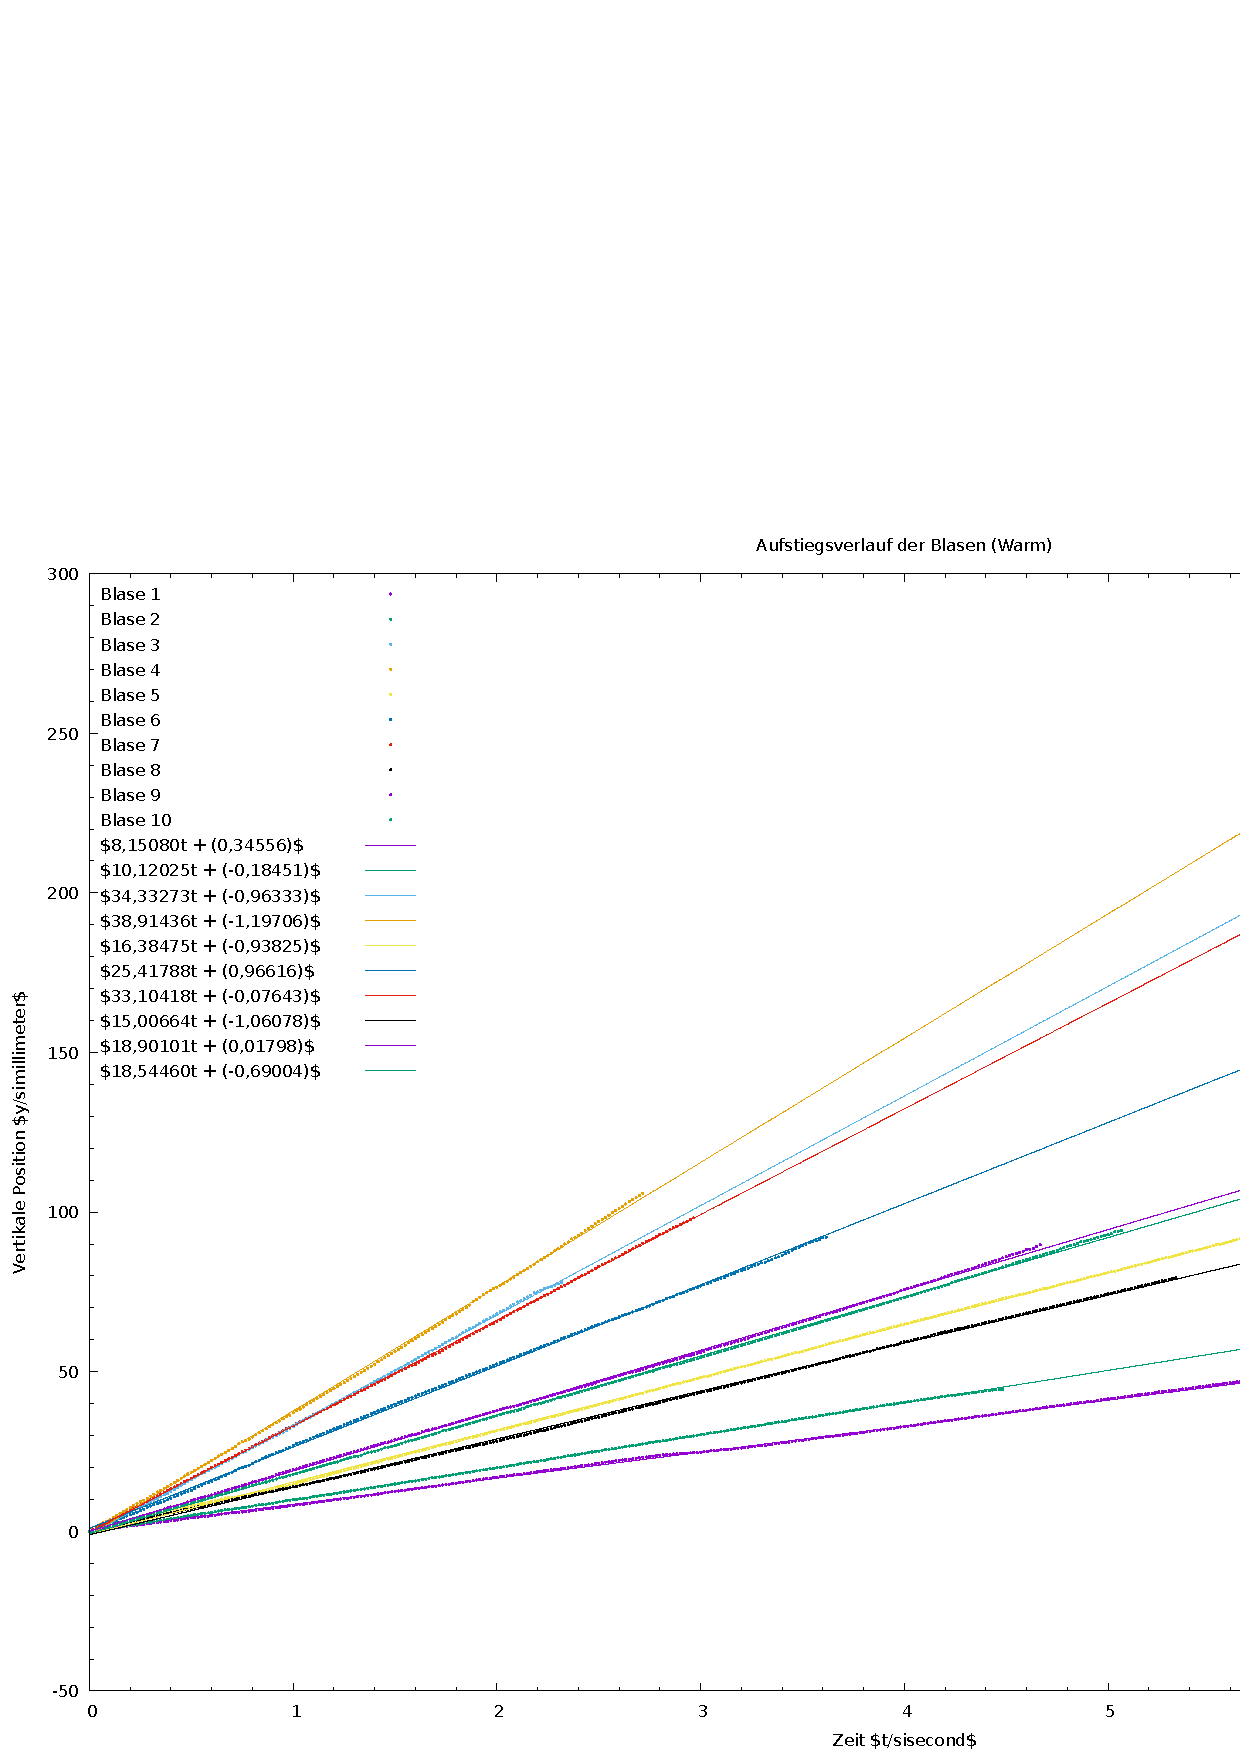
\includegraphics[width={432.00bp},height={288.00bp}]{tv1-plot}}%
    \gplfronttext
  \end{picture}%
\endgroup

		\caption{\centering Drehmoment auf stromdurchflossene Spule \captionbr $\chi^2_{\text{red}} = \num{0.0525026} \implies$ Gute Anpassung}
		\label{fig:tvone-plot}
		\vspace{-1em}
	\end{figure}
